\section{Einleitung}
Jeder nutzt es, sei es nur um spezielle Inhalte zu konsumieren, wie die Tagesschau oder ein Sportgroßereignis wie die Fußball Weltmeisterschaft oder die Olympischen Spiele.
Wegzudenken ist das TV aus der heutigen Gesellschaft nicht mehr. Es zählt zu einem der wichtigsten Medien.
Wie in jedem Bereich des täglichen Lebens erhählt die Digitalisierung als auch der Fortschritt mal mehr oder weniger schnell Einzug. Aber Sie kommt. In der vorliegenden Hausarbeit wird das Thema
''Streaming und Pay-TV'' betrachtet. \newline
Im speziellen behandelt diese Hausarbeit die Fragen nach den technischen Grundlagen für das Fernsehen über das Internet als auch für das Pay-TV.
Zusätzlich wird erläutert über welche technischen Erweiterungen der ''Conditional Access'' verfügbar ist.
Ebenso erörtert diese Hausarbeit, welche Auswirkunden und Konsequenzen sich für Zuschauer und Programmgestalter, seit und durch die Einführung der neuen oder anderen Möglichkeiten ergeben oder bereits ergeben haben.

\subsection{Zielsetzung}
Ziel dieser Arbeit ist es, Grundlagenwissen zu vermitteln. Ich zeige die grundsätzlichen Unterschiede zwischen dem klassischen ''linearen''--Fernsehen, dem Pay-TV und dem Konsum von Inhalten per Streaming auf.
Ich werde eine kleine Übersicht über die Diensteanbieter liefern ohne auf die Vor- als auch Nachteile der einzelnen Angebote einzugehen.


\subsection{Aufbau der Arbeit}
Das Kapitel 2 beeinhaltet die technischen Grundlagen der jeweiligen ''Bezugsquelle''. Im einzelnen gehe ich auf, erforderlich für das Streaming, die technische Übermittlung der Daten über das Internet ein. Ebenso erläutere ich die Unterschiede im DVB (Digital Video Broadcast), dort unterscheidet man drei Bezugsquellen und Techniken.
In Kapitel 3 werden die Begriffe Pay--TV (siehe Punkt 2.1), Streaming (siehe Punkt 2.2) und linearem-TV definiert und Unterschiede aufgezeigt.
Anschliessend folgt eine Zusammenfassung der Erkenntnisse um dann abschliessend mit dem Fazit einen kleinen Ausblick in die Zukunft zu geben. 









% \section{Einleitung}
% Dies soll eine \LaTeX{} -Vorlage für den persönlichen Gebrauch werden. Sie hat weder einen Anspruch auf Richtigkeit, noch auf Vollständigkeit. Die Quellen liegen auf Github zur allgemeinen Verwendung. Verbesserungen sind jederzeit willkommen.
%
% \subsection{Zielsetzung}
% Kleiner Reminder für mich in Bezug auf die Dinge, die wir bei der Thesis beachten sollten und \LaTeX{}-Vorlage für die Thesis.
%
% \subsection{Aufbau der Arbeit}
% Kapitel 2 enthält die Inhalte des Thesis-Days und alles, was zum inhaltlichen erstellen der Thesis relevant sein könnte. Kapitel 3 wichtige Anmerkungen zu \LaTeX{}, wobei die wirklich wichtigen Dinge im Quelltext dieses Dokumentes stehen.
%
% \begin{figure}[H]
% \begin{center}
% 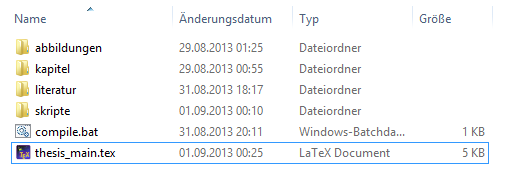
\includegraphics[width=0.9\textwidth]{verzeichnisStruktur}
% \caption{Verzeichnisstruktur der \LaTeX{}-Datein}
% \end{center}
% \end{figure}
